\section{Generating fuzzed data}

\begin{figure}[H]
    \centering
    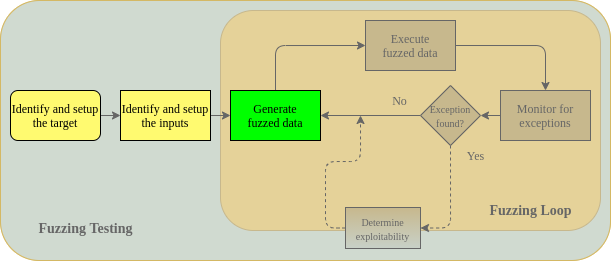
\includegraphics[width=\linewidth]{Chapter3/fuzzing_phase3.png}
\end{figure}

To generate new input files, Waffle takes the advantage of all three methods used by AFL, Memlock and SlowFuzz to cover more paths and to consider maximising the memory and instruction counters. Waffle has three phases for generating new input files and these phases are selected one after another (Figere \ref{fig:gen_phases}).

\begin{figure}[H]
    \centering
    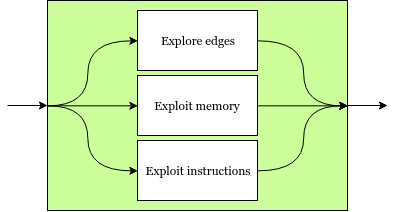
\includegraphics[width=0.8\linewidth]{Chapter3/gen_phases.png}
    \label{fig:gen_phases}
\end{figure}

Each one of the phases is selected with probabilities of $p_{e}$, $p_{em}$, and $p_{ei}$, which are for exploring edges, exploiting memory, and exploiting number of instructions, respectively.

Each phases defines it's own favored inputs:
\begin{itemize}
    \item \textbf{Explore edges:} As it is explained in \ref{eq:afl_fav_fac}
    \item \textbf{Exploit memory:} The bitmap for performance bits is first analyzed for any new discoveries. 
    \item \textbf{Exploit instructions:}
\end{itemize}

After a phase is finished, Waffle picks the inputs that are \textit{favored} and executes them in the next stage, executing the fuzzed data.

Compared to AFL, Waffle changes it's perspective for considering the favored inputs with a probability $p\_max\_counting$. 

\begin{equation}
    favored\_factor = perf\_bits[i]
\end{equation}

Waffle simplifies the selection of favorite inputs in order to continue the exploration for the maximum number of times a specific set of instructions are called. Waffle collects instruction counters into $perf\_bits[]$ and maximising the values in the cells of the array $perf\_bits$ is guiding the exploration of Waffle, in addition to the method AFL uses. 

Waffle continues the strategies of AFL for mutations and does not consider any modification in the mutation steps.

% Define what is favorable